\section{Resultados}
\subsection{Resultados de la evaluaci�n}
\begin{frame}
	\frametitle{Preguntas en lenguaje natural}
	%%%%%%%%%%%%%%%%%%%%%%%
	\begin{figure}
	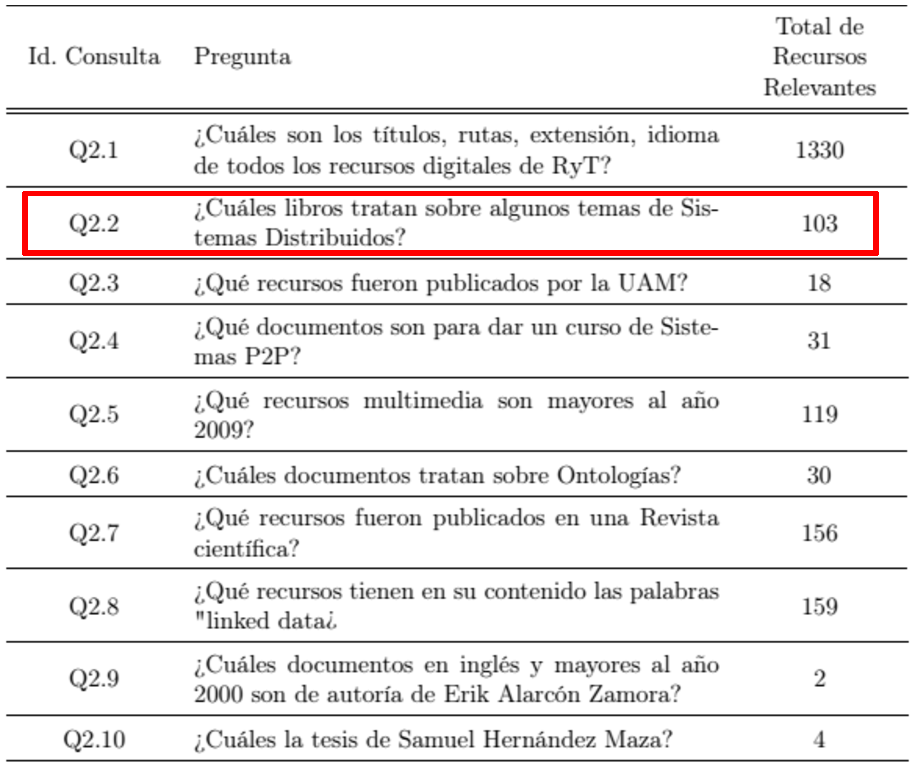
\includegraphics[scale=0.50]{Preguntas} 
	\end{figure}
\end{frame}

\begin{frame}
	\begin{block}{}
	Q2.2.- �Cu�les libros tratan sobre algunos temas de Sistemas Distribuidos?
	\end{block}

	\frametitle{Calidad en los Resultados}
	%%%%%%%%%%%%%%%%%%%%%%%
	\begin{figure}
	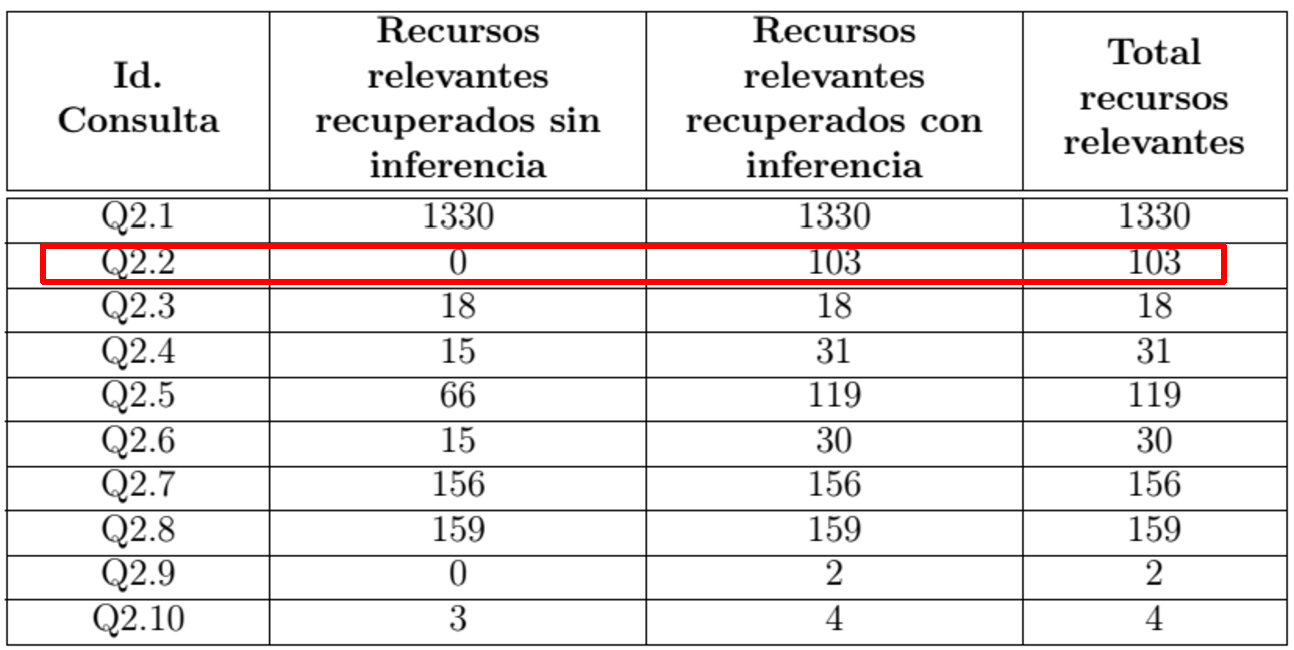
\includegraphics[scale=0.45]{Calidad} 
	\end{figure}
\end{frame}

\begin{frame}
	\frametitle{Tiempos de Procesamiento}
	%%%%%%%%%%%%%%%%%%%%%%%
	\begin{figure}
	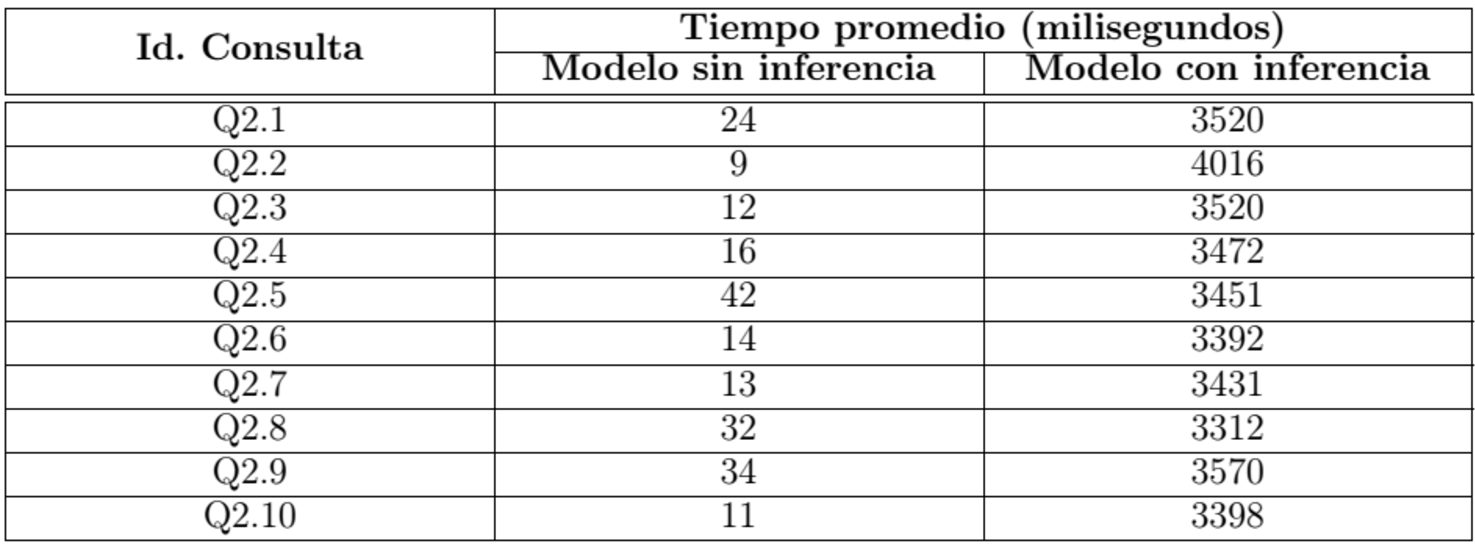
\includegraphics[scale=0.45]{Tiempos} 
	\end{figure}
\end{frame}

\subsection{Aportaciones}
\begin{frame}
	\frametitle{Aportaciones}
	\begin{enumerate}%[<+-| alert@+>]
	\item \justifying Un \textit{marco de referencia} para lograr la \textit{integraci�n sem�ntica} de \textit{recursos de informaci�n}.
    \item \justifying Un modelo sem�ntico que representa el conocimiento de una memoria corporativa.
    \item \justifying  Un prototipo (interfaz gr�fica de usuario) para la interacci�n amigable (b�squeda y consulta de informaci�n) de los usuarios con el modelo sem�ntico.
    \item \justifying Los resultados de nuestra evaluaci�n experimental.
    \item \justifying Un par de scripts para la generaci�n autom�tica y controlada de descripciones (conocimiento expl�cito) de los \textit{recursos de informaci�n}.
	\end{enumerate}
\end{frame}